\maketitle
%\thispagestyle{fancy}
\section*{Overview}

\subsection*{Goals}

Our goals for this month were as follows: 

\begin{itemize}
  \item 
    Identify concrete objective functions for the Swarm incentive system with a view to multi-objective optimisation.
  \item
    Study the convergence of system state on allocatively efficient equilibria.
  \item
    Inspect historic activity in the Swarm stake registry and look for evidence of competitive behaviour.
\end{itemize}

\subsection*{Methodology}

We used a classical microeconomic equilibrium approach to formulating abstract objectives for the Swarm economy, then mechanism design to interpret the supply function in terms of the actual redistribution game.

For studying activity on the stake registry, we pulled historic log data from the stake registry contract, matched block numbers with known significant network events to pick suitable date ranges, and built a Python notebook to calculate basic statistics and create visualisations.\footnote{\url{https://github.com/shtukaresearch/swarm-staking/blob/main/marimonb/swarm-data.py}}

\subsection*{Scope}

We formulated the objectives using a minimal supply-and-demand model for Swarm storage where the details of the redistribution mechanism is abstracted away.
%
For evaluating a specific iteration of Swarm against these objectives, we used the storage incentive system deployed between versions 0.6.0 and 0.9.1.\footnote{The changes introduced in the new Redistribution contract deployed in v0.8.6 are out of scope for our model.}

The observational study focused on the version of the stake registry bundled with v0.4.0 of the storage incentive system (deployed block 25,527,075) and deprecated with v0.9.1 (block 35,961,749).
%
For more details, see \textbf{Findings}.

\section*{Operations management}

\subsection*{Completed Milestones}

\begin{itemize}
  \item 
    Expand on candidate list of quantitative objectives for the Swarm staking system.
  \item 
    Develop stochastic perfect information model that captures core aspects of the current staking system. 
    %
    Use solutions to the deterministic model to back out results that hold in expectation.

  \item Study staker decision processes and risks without the assumptions of determinism.
  
  \item Establish conditions for market clearing at the target replication rate.
  
  \item Identify aggregate economic indicators and metrics relevant for monitoring and forecasting Swarm storage performance and making decisions about improvements.

  
  \item Pull data on historic staker behaviour and analyse it in the context of our model. Are there any stakers that already exhibit strategic behaviour? How frequent are instances of direct competition in acquiring stake positions? Create visualisations.
\end{itemize}

\subsection*{Future milestones}

\begin{itemize}
  \item Compile formal report and executive summary.
\end{itemize}

\subsection*{Revised milestones}

\begin{itemize}
  \item Numerical solution of Bellman equation for $n$-step strategies in the stochastic setting. 
  
  In the September report, it was claimed that optimal $n$-step policies terminate in one step under perfect information and stationarity.
  %
  This is not true.
  %
  However, due to time constraints we propose to defer numerical estimation of these policies to a future project.

  
  \item Study staker decision processes without the assumptions of complete information or stationarity. Due to time constraints, this will have to be left to a future project.

\end{itemize}


\subsection*{Schedule}

\paragraph{November} Compile formal LaTeX report. Gather recommendations and compose roadmap for future research.

\paragraph{December} \emph{fin}




\newpage
\section*{Findings}

\subsection*{Summary}

\begin{itemize}
  \item Multi-objective optimisation
  \item Microeconomic equilibrium
  \item Efficiency and reallocation events
  \item Observational studies
\end{itemize}

\subsection*{Microeconomic equilibrium }

We revised and clarified our approach to defining system design objectives, identifying specific objective functions and studying their implementation through a mechanism design approach.
%
The key objective functions under study this month were:
\begin{enumerate}
  \item Maximise sales (growth) subject to QoS constraints;
  \item Minimise storage price subject to QoS constraints;
  \item Maximise QoS at a given price.
\end{enumerate}
For the third criterion, we evaluate QoS purely in terms of replication rate, which the design of the Swarm protocol calls for having a target value of $4$.\footnote{Presumably, if a strictly higher replication rate can be provided for the same or lower price, this would also be fine.}

If we write $\mathcal{D}=\uR$ for demand space, $\mathcal{P}=\uR$ for price space, and $\mathcal{Q}=\uR$ for QoS (replication rate) space, then the Swarm protocol rules and exogenous world state determines a set of feasible allocations
%
\[
  X \subset \mathcal{D}\times\mathcal{P}\times\mathcal{Q}.
\]
%
Here, a point $(D,p,q)$ is \emph{feasible} if the realised revenue $R=pD$ can be distributed among a population of storage providers \emph{in some way} such that they would collectively be prepared to meet the demand $D$ with replication rate $q$, i.e.~provide $pD$ units of storage.
%
The means by which this distribution is achieved is within the purview of the Swarm protocol designers.

Classical demand theory tells us that for any $q\in \mathcal{Q}$, the feasible slice 
\[
  X_q = X \cap (\mathcal{D}\times\mathcal{P}\times\{q\})
\]
is a downward-sloping curve in the positive quadrant $\uR^2$.
%
That is, the storage price is minimised within the feasible region if and only if demand is maximised.

To transform this optimisation problem into one parametrised over price, where $q$ may vary, we look for a selection rule 
\[
  \xi^*:\mathcal{P}\rightarrow X\cup\{\bot\}
\]
that assigns a feasible state $\xi^*(p)=(D^*,p,q^*)\in X\cap \mathcal{D}\times\{p\}\times\mathcal{Q}$ such that $q^*$ is maximal in $X\cap \mathcal{D}\times\{p\}\times\mathcal{Q}$.
%
Classical supply theory tells us that $q^*(p)$ is \emph{increasing} in $p$. 
%
Then the price objective can be achieved by finding the minimal $p$ such that $q^*(p)\geq 4$; if $q^*$ is strictly increasing in $p$, continuous, and $q^*(0)=0$, then this minimum achieves the target rate $q^*=4$.

\paragraph{Implementing the optimal allocation}
The mechanism design approach to economic management tells us to search for a \emph{redistribution mechanism} 
\[
  \mathbf{M}:\uR \times \Xi \rightarrow \uR^\Overlay
\]
together with a (Bayes-Nash) equilibrium $\xi^*(R)\in\Xi$.
%
where $\uR$ is revenue space, $\Xi$ is some endogenous state space, and $\Overlay$ is the address space of NOs.
%
We require that $\sum\mathbf{M}(R,\xi)\leq R$, that is, the mechanism is within budget.

The endogenous state space can take several forms, but we ask that it at least record whether each node is \emph{active} via a map $\mathtt{on}:\Xi\rightarrow \{\bot,\top\}^\Overlay$.
%
Then we can define the \emph{replication rate} of the equilibrium $\xi^*$ by the formula
\[
  q(\xi^*) = \sum\mathtt{on}(\xi^*);
\]
say also that $(\mathbf{M},\xi^*)$ \emph{implements} $q$.

\begin{example*}In the version of the Swarm mechanism under consideration, the endogenous state vector $\xi^*$ consists of a mapping $(\mathtt{on},x):\Overlay\rightarrow \{\bot,\top\}\times\uR$ that identifies whether a node is active and what their equity balance is.
\end{example*}

\paragraph{Identifying an optimal allocation}
Suppose we have access to the variable costs $O:\Overlay\rightarrow\uR$ of each NO, that is, the cost of providing a single active node.
%
For simplicity, we assume that $O$ does not depend on the quantity of storage provided; this is not as ridiculous as it sounds if we assume that NOs must reserve a certain amount of computation to run their node, regardless of how full the reserve is, and that realised demand does not stray past a power of two, triggering a neighbourhood split.
%
Finally, we assume that $\Overlay\subseteq\N$ is well-ordered and that $O(a)$ is increasing in $a$, i.e.~the node addresses are sorted in order of increasing operating cost.

The following result is not hard to prove:
%
\begin{proposition*}
  Under the above assumptions, let $K\in\Overlay$ be the maximum index such that
  \[
    \sum_{k=0}^KO(k) \leq R.
  \]
  Then the redistribution weights
  \[
    w_k = \left\{ \begin{array}{ll}
      O(k)/\sum_{i=0}^KO(i) & k\leq K \\
      0 & k > K
    \end{array} \right.
  \]
  define a QoS-optimal allocation with replication rate $K$.
\end{proposition*}

The Swarm protocol does not have direct access to the quantities $O(a)$, so the preceding mechanism cannot be implemented as stated.
%
Instead, Swarm needs to provide some kind of market where would-be NOs can express their costs indirectly through market positioning.

\paragraph{Does the Swarm redistribution mechanism implement $(p^*(4),4)$?}

No, it does not.

\newpage
\subsection*{Observational studies}

Are NOs behaving competitively in the staking game?
%

Significant dates:
\begin{itemize}
  \item September 21st, 2023. Bee node version 1.17.4 drops, introducing the \texttt{--target-neighborhood} option.
  \item October--November, 2023. Over 16,000 new active nodes appear in China, quintupling the total number of active nodes in the network. Half of these become inactive after November.
  \item May 2024. 11-bit replication neighbourhoods become common.
\end{itemize}

\paragraph{Observation period}
We drew observations from the deployment of v0.4.0 of the stake registry contract in block 25,527,075 until its pausing in block 35,963,617.\footnote{It might make sense to cut things off at the slightly earlier time of block 35,961,749, when version 0.9.1 of the stake registry contract incorporating rules from SWIP-19 and SWIP-20 was deployed, but since the difference was just 2 hours and 20 minutes, we ignore this.} This represents about 2 years of network activity

We noticed substantial staking activity among new overlay addresses in October and November of 2023, presumably an impact of the thousands of new active nodes that reportedly appeared in China during this period.\footnote{\url{https://blog.ethswarm.org/foundation/2024/state-of-the-network-january/}}
%
We sampled this outlier event out of the data by only considering blocks starting at 31,000,000, around mid-November, by which time the main cluster of updates was complete.

\paragraph{Binning} We gathered addresses into neighbourhoods assuming that the bit depth is 10.

\paragraph{Summary statistics}
All 1024 bins in the 10-bit address space saw events during the observation period.
%
In total, 5360 overlay addresses were observed.

\begin{table}
  \hfill
  \begin{tabular}{cc}
    \multicolumn{2}{l}{Addresses per bin} \\
    \toprule 
    mean      & 5.23 \\
    $\sigma$  & 7.84 \\
    max       & 178 \\
    min       & 1  \\
    \bottomrule
  \end{tabular}
  \hfill
  \begin{tabular}{cc}
    \multicolumn{2}{l}{Events per bin} \\
    \midrule 
    mean      & 6.04 \\
    $\sigma$  & 7.96 \\
    max       & 178 \\
    min       & 1 \\
    \bottomrule
  \end{tabular}
  \hfill
  \begin{tabular}{cc}
    \toprule
    \multicolumn{2}{l}{Events per address}\\
    \midrule
    mean      & 1.15 \\
    $\sigma$  & 0.55 \\
    max       & 8\footnote{Achieved at address {\tiny\texttt{0x720c3...8736}}}  \\
    \bottomrule
  \end{tabular}
  \hfill
  %
  \caption{
    Statistics of events and addresses
  }  
\end{table}

The maximum number of events per bin (resp.~per address) was achieved on bin \texttt{0b0011001010} (resp.~address {\tiny\texttt{0x720c3...8736}}).

\paragraph{Contested neighbourhoods}
We define a bin to be:
\begin{enumerate}
  \item \emph{weakly contested} if it has more stake update events than addresses in the observation period;
  \item \emph{contested} if it contains at least one stake update event that \emph{revisits} its address in the sense that its address was observed in a previous event, but not the previous event.
\end{enumerate}
The ``definition of contested'' is intended to capture a dynamic of at least two addresses cycling back and forth topping up their equity accounts; the implicit assumption being that such behaviour is \emph{reactive} and hence strategic.

We found 395 weakly contested bins and 149 contested bins. 
%
The stake update events in the first (lexicographically ordered) 54 contested bins are displayed in the plot below.


\begin{center}
\begin{figure}[p]
  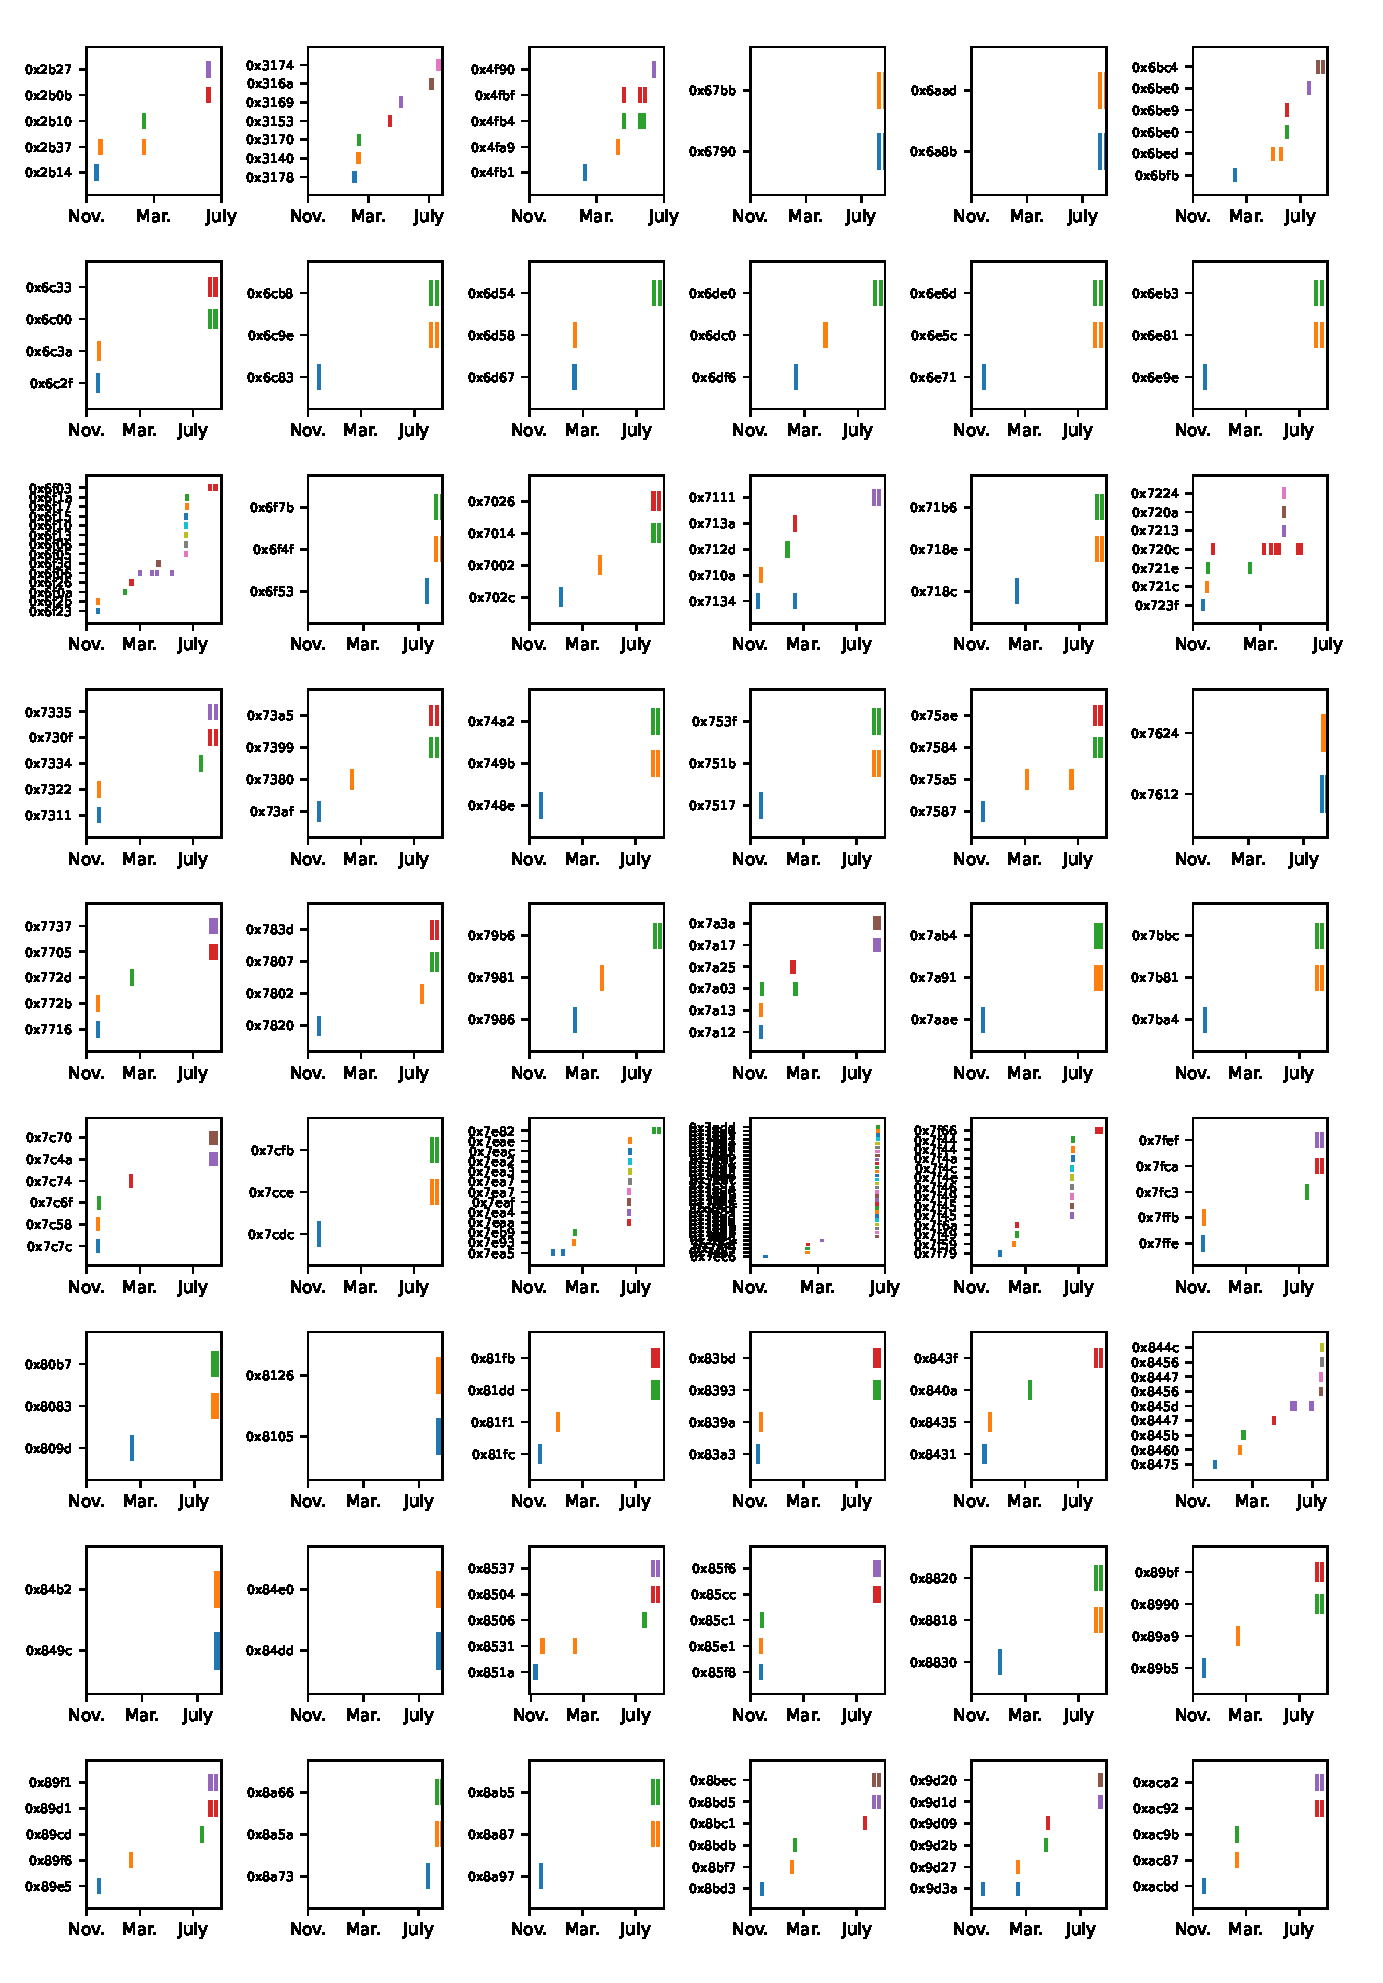
\includegraphics[width=\textwidth]{common/contested.eps}
  \caption{Stake update events in contested neighbourhoods}
  \label{event-plot}
\end{figure}
\end{center}


On many of the plots we can observe pairs of addresses that repeatedly top up at very similar times to one another.
%
For example, check this out from the {\texttt{0x6c8}} bin (the eighth plot in Figure \ref{event-plot}):
%
\begin{center}
\begin{tabular}{lll}
Date + time         & Address & Amount (BZZ) \\
\hline
2023-11-21 19:40:00 & 0x6c83 &   11 \\
2024-07-23 22:15:50 &	0x6c9e  &	10 \\
2024-07-23 22:16:05 &	0x6cb8  &	10 \\
2024-08-04 21:56:25 &	0x6c9e  &	10 \\
2024-08-04 21:56:45 &	0x6cb8  &	10
\end{tabular}
\end{center}
%
We posit that the most likely reason for this behaviour is that the same entity started numerous nodes at the same time and placed them in distinct 11-bit neighbourhoods.
%
Since we have sorted by 10-bit neighbourhoods we have caught multiple of these nodes in the same bin, making their activity look like contention.